\author[Zahari Kassabov]{}
\institute{University of Cambridge}

\begin{frame}{Why can't we fit a dataset?}
\protect\hypertarget{why-cant-we-fit-a-dataset}{}
Three possibilities:

\begin{enumerate}
\tightlist
\item
  Problems with the experiment
\item
  Problems with the theory (including methodology)
\item
  Tension with other dataset (i.e.~1. or 2. but for other data)
\end{enumerate}

\textbf{Objective}: Investigate the origin of issue

\textbf{Tool: Constrained fits}; Try to constrain the fit to agree with
the dataset under investigation and see what breaks in the process.
\end{frame}

\begin{frame}{Implementation}
\protect\hypertarget{implementation}{}
Idea from \emph{Why \(\alpha_s\) Cannot be Determined from Hadronic
Processes without Simultaneously Determining the Parton Distributions}
{[}Forte, Z.K.,
\href{https://arxiv.org/abs/2001.04986}{\textbf{arxiv:2001.04986}}{]}

Instead of optimizing for the total \(\chi^2\), give special attention
to the agreement of the dataset under investigation by giving more
weight to its error \(\chi^2_p\).

\[
\chi^2 + w \chi^2_p
\] where \(w\) is \emph{big}.

Consequences, compared to optimizing for \(\chi^2\):

\begin{itemize}
\tightlist
\item
  Total \(\chi^2\) will go up, because we are not optimizing for it any
  longer.

  \begin{itemize}
  \tightlist
  \item
    Observe which datasets get worse ans how much: Assess \textbf{3}.
  \end{itemize}
\item
  Dataset error, \(\chi^2_p\) will go down.

  \begin{itemize}
  \tightlist
  \item
    Observe if we can reasonably get a good agreement or the dataset is
    not self consistent. Conclude \textbf{1} or \textbf{2}, but likely
    \textbf{1} as our methodology is \emph{very} flexible
  \end{itemize}
\end{itemize}
\end{frame}

\begin{frame}{Example: DO electron Asymmetry}
\protect\hypertarget{example-do-electron-asymmetry}{}
We cannot fit the D0 electron assymetry dataset. Set $w=411$.

\tiny
\begin{longtable}[]{@{}lll@{}}
\toprule
\begin{minipage}[b]{0.19\columnwidth}\raggedright
\(\chi^2\)/ndat\strut
\end{minipage} & \begin{minipage}[b]{0.14\columnwidth}\raggedright
Baseline\strut
\end{minipage} & \begin{minipage}[b]{0.28\columnwidth}\raggedright
Reweighted D0EASY\strut
\end{minipage}\tabularnewline
\midrule
\endhead
\begin{minipage}[t]{0.19\columnwidth}\raggedright
D0 e ASY\strut
\end{minipage} & \begin{minipage}[t]{0.14\columnwidth}\raggedright
5.3\strut
\end{minipage} & \begin{minipage}[t]{0.28\columnwidth}\raggedright
1.7\strut
\end{minipage}\tabularnewline
\begin{minipage}[t]{0.19\columnwidth}\raggedright
D0 \(\mu\) ASY\strut
\end{minipage} & \begin{minipage}[t]{0.14\columnwidth}\raggedright
2.0\strut
\end{minipage} & \begin{minipage}[t]{0.28\columnwidth}\raggedright
5.4\strut
\end{minipage}\tabularnewline
\begin{minipage}[t]{0.19\columnwidth}\raggedright
Total\strut
\end{minipage} & \begin{minipage}[t]{0.14\columnwidth}\raggedright
1.17\strut
\end{minipage} & \begin{minipage}[t]{0.28\columnwidth}\raggedright
1.29\strut
\end{minipage}\tabularnewline
\bottomrule
\end{longtable}
\vspace{-1.5em}

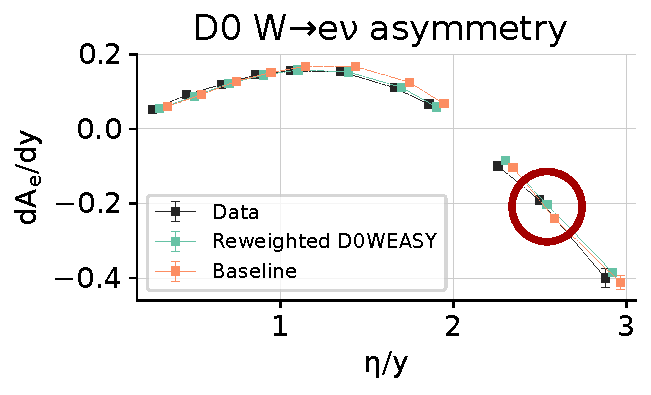
\includegraphics[width=0.45\textwidth,height=0.26\textwidth]{weight_fits/plots/D0WEASY_Norm1_plot_fancy_0.pdf}
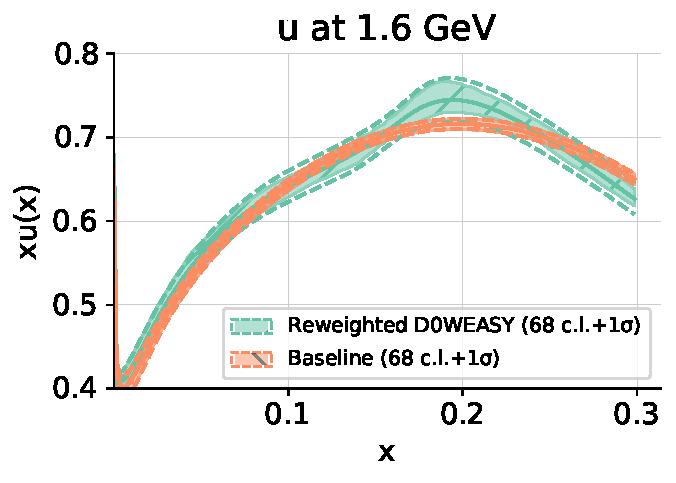
\includegraphics[width=0.45\textwidth,height=0.26\textwidth]{weight_fits/plots/plot_pdfs_u.pdf}
\normalsize


\vspace{-1em}

\begin{itemize}
\tightlist
\item
  Can lift the downward prediction but only at the cost of:

  \begin{itemize}
  \tightlist
  \item
    Introducing unnatural shapes
  \item
    Increasing error in other datasets particularly D0 \(\mu\)
    asymmetry.
  \end{itemize}
\item
  The large weight fit still obtains poor fit quality for D0EASY:

  \begin{itemize}
  \tightlist
  \item
    \textbf{Dataset not self consistent}.
  \end{itemize}
\end{itemize}
\end{frame}
